\section{OpenCV}
OpenCV adalah kumpulan pustaka untuk bidang {\em computer vision}
atau {\em image processing}.
Pustaka ini dapat diakses dengan menggunakan bermacam-macam bahasa pemrograman,
termasuk bahasa Python.
Untuk memasang pustaka atau modul ini gunakan perintah.

\begin{verbatim}
pip install opencv-python
\end{verbatim}

Berikut ini adalah sebuah contoh penggunaan OpenCV untuk membaca
sebuah berkas gambar dan mengubahnya warnanya menjadi abu-abu (greyscale).
Perhatikan nama berkas yang dalam contoh ini berada di direktori
satu tingkat di atasnya. Ganti nama berkas ini dengan nama yang sesuai
dengan berkas yang ingin Anda proses.

\begin{verbatim}
import cv2
img = cv2.imread('../graphics/br-pixel.png')
grey = cv2.cvtColor(img, cv2.COLOR_BGR2GRAY)
cv2.imshow('Gambar Asli', img)
cv2.imshow('Gambar grey', grey)
cv2.waitKey(0)
cv2.destroyAllWindows()
\end{verbatim}

Program akan menampilkan gambar sebelum dan sesudah diproses,
kemudian menunggu sampai kita menekan sesuatu di keyboard sebelum
akhirnya menutup semua peragaan gambar tersebut.
Hasil pemrosesan kode di atas dapat dilihat pada gambar-gambar
berikut.

\begin{figure}

\includegraphics[width=1.0\linewidth]{graphics/br-pixel.png}
\caption{Gambar asli}
\end{figure}

\begin{figure}
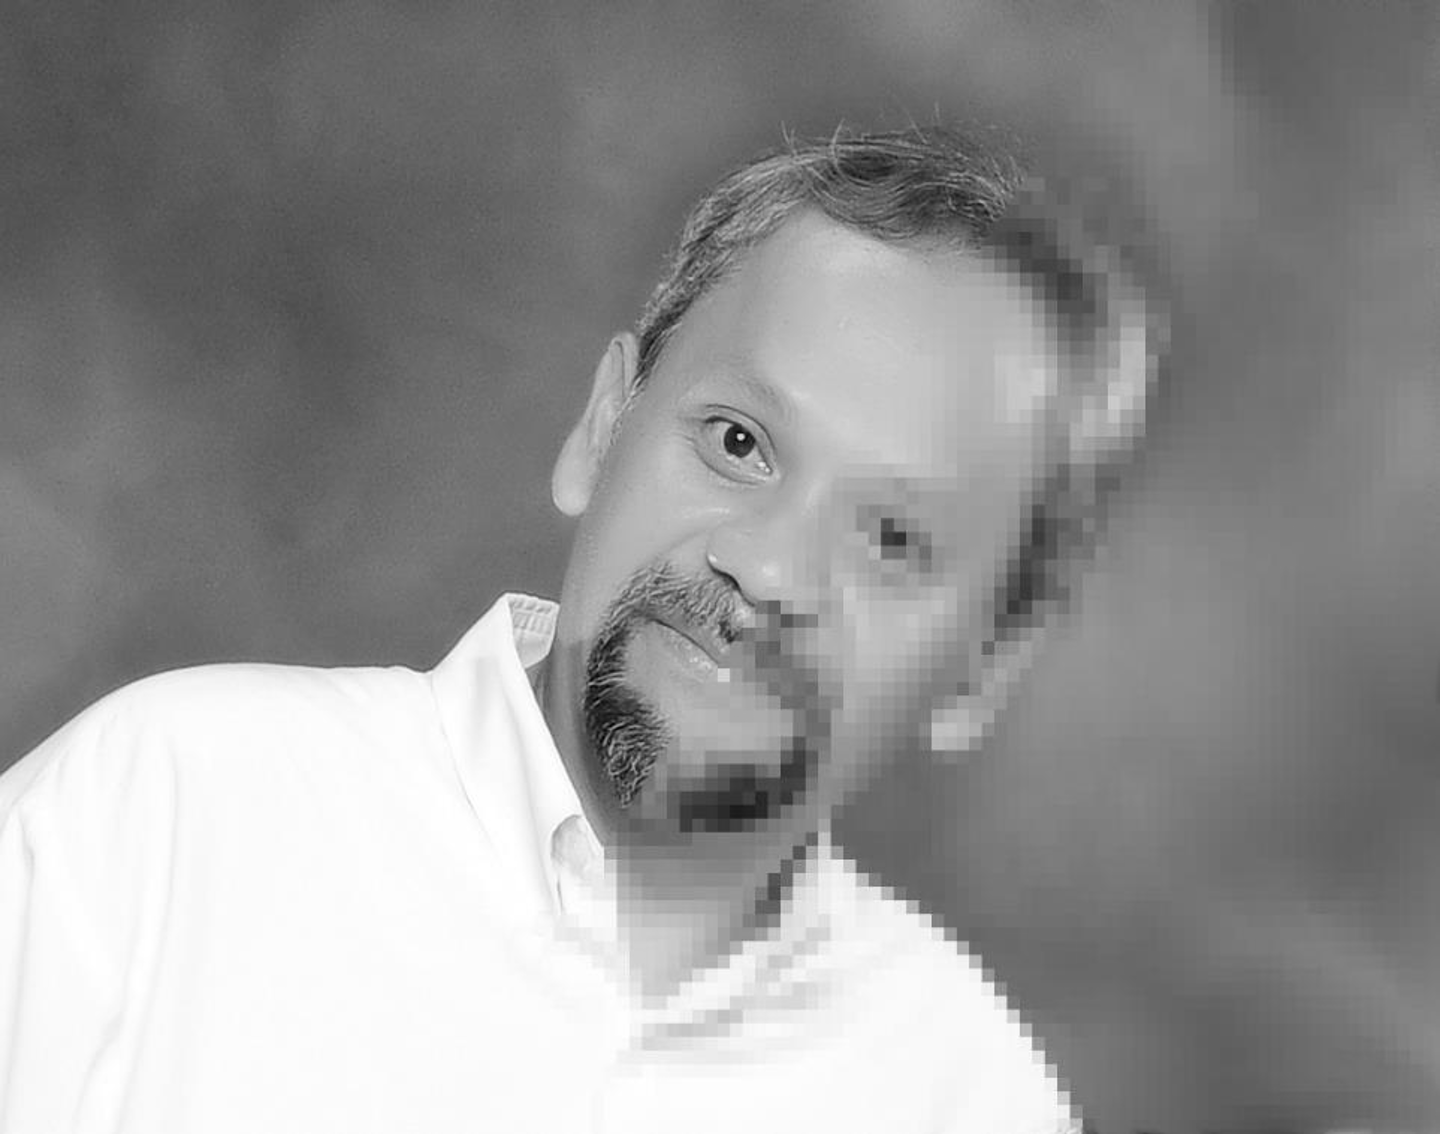
\includegraphics[width=1.0\linewidth]{graphics/br-pixel-grey.png}
\caption{Hasil proses}
\end{figure}

Modul OpenCV ini dapat digunakan di berbagai aplikasi, termasuk untuk
Artificial Intelligence atau Machine Learning.
